% *======================================================================*
%  Cactus Thorn template for ThornGuide documentation
%  Author: Ian Kelley
%  Date: Sun Jun 02, 2002
%  $Header$
%
%  Thorn documentation in the latex file doc/documentation.tex
%  will be included in ThornGuides built with the Cactus make system.
%  The scripts employed by the make system automatically include
%  pages about variables, parameters and scheduling parsed from the
%  relevant thorn CCL files.
%
%  This template contains guidelines which help to assure that your
%  documentation will be correctly added to ThornGuides. More
%  information is available in the Cactus Users Guide.
%
%  Guidelines:
%   - Do not change anything before the line
%       % START CACTUS THORNGUIDE",
%     except for filling in the title, author, date, etc. fields.
%        - Each of these fields should only be on ONE line.
%        - Author names should be separated with a \\ or a comma.
%   - You can define your own macros, but they must appear after
%     the START CACTUS THORNGUIDE line, and must not redefine standard
%     latex commands.
%   - To avoid name clashes with other thorns, 'labels', 'citations',
%     'references', and 'image' names should conform to the following
%     convention:
%       ARRANGEMENT_THORN_LABEL
%     For example, an image wave.eps in the arrangement CactusWave and
%     thorn WaveToyC should be renamed to CactusWave_WaveToyC_wave.eps
%   - Graphics should only be included using the graphicx package.
%     More specifically, with the "\includegraphics" command.  Do
%     not specify any graphic file extensions in your .tex file. This
%     will allow us to create a PDF version of the ThornGuide
%     via pdflatex.
%   - References should be included with the latex "\bibitem" command.
%   - Use \begin{abstract}...\end{abstract} instead of \abstract{...}
%   - Do not use \appendix, instead include any appendices you need as
%     standard sections.
%   - For the benefit of our Perl scripts, and for future extensions,
%     please use simple latex.
%
% *======================================================================*
%
% Example of including a graphic image:
%    \begin{figure}[ht]
%       \begin{center}
%          \includegraphics[width=6cm]{MyArrangement_MyThorn_MyFigure}
%       \end{center}
%       \caption{Illustration of this and that}
%       \label{MyArrangement_MyThorn_MyLabel}
%    \end{figure}
%
% Example of using a label:
%   \label{MyArrangement_MyThorn_MyLabel}
%
% Example of a citation:
%    \cite{MyArrangement_MyThorn_Author99}
%
% Example of including a reference
%   \bibitem{MyArrangement_MyThorn_Author99}
%   {J. Author, {\em The Title of the Book, Journal, or periodical}, 1 (1999),
%   1--16. {\tt http://www.nowhere.com/}}
%
% *======================================================================*

% If you are using CVS use this line to give version information
% $Header$

\documentclass{article}

% Use the Cactus ThornGuide style file
% (Automatically used from Cactus distribution, if you have a
%  thorn without the Cactus Flesh download this from the Cactus
%  homepage at www.cactuscode.org)
\usepackage{../../../../doc/latex/cactus}

\begin{document}

% The author of the documentation
\author{Erik Schnetter \textless schnetter@aei.mpg.de\textgreater}

% The title of the document (not necessarily the name of the Thorn)
\title{SymBase}

% the date your document was last changed, if your document is in CVS,
% please use:
\date{$ $Date$ $}

\maketitle

% Do not delete next line
% START CACTUS THORNGUIDE

% Add all definitions used in this documentation here
%   \def\mydef etc

% Add an abstract for this thorn's documentation
\begin{abstract}
When the computational domain has symmetries, then it is often very
convenient to be able to interpolate at points that are not present on
the actual computational grid, but can be mapped into the grid through
the symmetries.  Thorn SymBase provides a mechanism by which symmetry
conditions can register routines that handle this mapping when a
global interpolator is called. 

\end{abstract}

% The following sections are suggestive only.
% Remove them or add your own.



\section{Introduction}

Thorn SymBase contains a registry for symmetry conditions and for
symmetry faces.  Other thorns that implement symmetry boundary
conditions register themselves with SymBase and reserve certain
faces of the grid, so that no other boundary condition is applied
there.  Thorns that implement physical boundary conditions should
query SymBase about the set of faces that have symmetry boundary
conditions and should not apply the physical boundary condition there.

\begin{figure}[ht]
\begin{center}
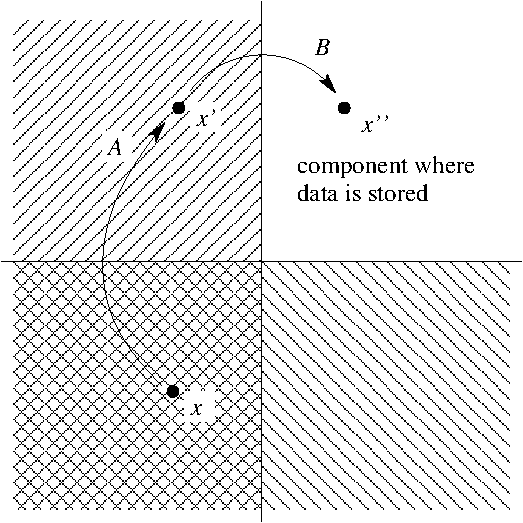
\includegraphics[scale=.833,clip=true]{fig/faces}
\end{center}
\caption[Symmetry transformations across faces] {
	Multiple SymBase symmetry transformations across
	different registered symmetry faces.

	A point $x$ is transformed to point $x'$ by transformation
	$A$, and then to point $x''$ by transformation $B$.  Data is
	only actually stored for point $x''$.
}
\label{SymBase.faces}
\end{figure}

The driver has to be aware that it calls thorn SymBase's mapping
routine before it actually interpolates.  The whole mechanism is
transparent for the user.



\section{Registering Symmetry Conditions}
\label{SymBase.registering_symmetry_conditions}

Each thorn that implements a symmetry boundary condition should
register itself with thorn SymBase.  This has no consequences per se,
but it reserves a \emph{symmetry handle} for later reference. 
The API for registering and querying symmetry names and handles is

\begin{verbatim}
CCTK_INT FUNCTION
    SymmetryRegister (CCTK_STRING IN sym_name)

CCTK_INT FUNCTION
    SymmetryHandleOfName (CCTK_STRING IN sym_name)

CCTK_POINTER_TO_CONST FUNCTION
    SymmetryNameOfHandle (CCTK_INT IN sym_handle)
\end{verbatim}

The routine \texttt{SymmetryRegister} should be called in a routine
that has been scheduled in the schedule group
\texttt{SymmetryRegister}.

\begin{quote}
Note: We have the API in the specification, we have it in the
interface file, in the source code, and in a header file, and I
duplicated it into grdoc headers.  I refuse to write and describe and
cross-check the API a \emph{sixth} time in latex.  At some point, we
have to start using tools for that.  Please read the grdoc headers or
the grdoc-produced HTML files for a detailed description.
\end{quote}



\section{Registering Symmetries for Faces}

Thorn SymBase keeps two registries.  The first, mentioned in the
previous section, is the set of symmetry boundary conditions. 
The second, the \emph{symmetry table}, prescribes to which faces
of the grids which symmetry boundary condition is to be applied.
Each entry of this table constitutes a mapping from grid faces to
symmetry boundary conditions, described by arrays whose elements
correspond to grid faces:

\begin{verbatim}
CCTK_INT symmetry_handle[]
CCTK_INT symmetry_zone_width[]
\end{verbatim}

The faces are numbered in the same way those of the \texttt{cctk\_bbox} array. 
Each element of \texttt{symmetry\_handle} is a symmetry handle as
described in section~\ref{SymBase.registering_symmetry_conditions}. 
The \emph{symmetry zone} is the same as a Cactus ghost zone, just in the
context of a symmetry boundary, so the \texttt{symmetry\_zone\_width} will
be typically be the same as the ghost zone width.

%Code outside SymBase should not modify these table entries.

There is one such table for the grid hierarchy, which is valid for all
grid functions.  There is additionally one such table for each grid
array group.

The API for registering symmetries for faces is

\begin{verbatim}
CCTK_INT FUNCTION
    SymmetryRegisterGrid
         (CCTK_POINTER IN cctkGH,
          CCTK_INT IN sym_handle,
          CCTK_INT IN ARRAY which_faces,
          CCTK_INT IN ARRAY symmetry_zone_width)

CCTK_INT FUNCTION
    SymmetryRegisterGI
        (CCTK_POINTER IN cctkGH,
         CCTK_INT IN sym_handle,
         CCTK_INT IN ARRAY which_faces,
         CCTK_INT IN ARRAY symmetry_zone_width,
         CCTK_INT IN group_index)

CCTK_INT FUNCTION
    SymmetryRegisterGN
        (CCTK_POINTER IN cctkGH,
         CCTK_INT IN sym_handle,
         CCTK_INT IN ARRAY which_faces,
         CCTK_INT IN ARRAY symmetry_zone_width,
         CCTK_STRING IN group_name)
\end{verbatim}

The first routine registers a symmetry condition for the grid hierarchy;
the other two routines register for grid array groups (by index or 
name, respectively)
\texttt{sym\_handle} must be a symmetry handle obtained as
described in the previous section.  \texttt{which\_faces} and
\texttt{symmetry\_zone\_width} are arrays with one element per face,
numbered in the same way as the \texttt{cctk\_bbox} array.
\texttt{which\_faces} selects which faces to register, and
\texttt{symmetry\_zone\_width} sets the number of symmetry zones for
these faces.

These routines may be called at anytime after \texttt{SymmetryRegister}.

It is not possible to register multiple symmetry boundary conditions
for the same face.



\section{Querying Symmetries of Faces}

Physical boundary conditions need to know to which faces they should
apply the boundary condition.  They need to query SymBase for the set
of faces that have a symmetry boundary condition, and they must not
apply their physical boundary condition there.  The API is

\begin{verbatim}
CCTK_INT FUNCTION
    SymmetryTableHandleForGrid (CCTK_POINTER_TO_CONST IN cctkGH)

CCTK_INT FUNCTION
    SymmetryTableHandleForGI
        (CCTK_POINTER_TO_CONST IN cctkGH,
         CCTK_INT IN group_index)

CCTK_INT FUNCTION
    SymmetryTableHandleForGN
        (CCTK_POINTER_TO_CONST IN cctkGH,
         CCTK_STRING IN group_name)
\end{verbatim}

The first of these functions returns the symmetry table handle for the
grid hierarchy; the second and third return the that for the grid array group
(by index or name, respectively).

The table entry with key \texttt{symmetry\_handle} contains the symmetry
handle for the symmetry boundary condition, or a negative number if the face
has no symmetry boundary condition associated with it.

The code to find out which boundaries should have a physical boundary
condition applied might look as follows:

\begin{verbatim}
#include "cctk.h"
#include "util_Table.h"

CCTK_INT symtable;
CCTK_INT symbnd[6];
int face;
int ierr;

symtable = SymmetryTableHandleForGrid (cctkGH);
if (symtable<0)
  CCTK_VWarn(0, __LINE__, __FILE__, "Thorn_Name", "symtable is out of bounds");

ierr = Util_TableGetIntArray (symtable, 6, symbnd, "symmetry_handle");
if (ierr!=6)
  CCTK_VWarn(0, __LINE__, __FILE__, "Thorn_Name", "Util_TableGetIntArray returned error");

for (face=0; face<6; ++face) {
  if (cctk_bbox[face] && symbnd[face]<0) {
    /* Apply physical boundary condition here */
  }
}
\end{verbatim}

\hrule

\begin{verbatim}
#include "util_Table.h"

CCTK_INT symtable
CCTK_INT symbnd(6)
integer face
integer ierr

symtable = SymmetryTableHandleForGrid (cctkGH)
if (symtable<0) call CCTK_WARN (0, "internal error")

call Util_TableGetIntArray (ierr, int(symtable), 6, symbnd, "symmetry_handle")
if (ierr/=6) call CCTK_WARN (0, "internal error")

do face=1,6
  if (cctk_bbox(face)/=0 .and. symbnd(face)<0) then
    ! Apply physical boundary condition here
  end if
end do
\end{verbatim}



\section{Symmetry Interpolation}

The mechanism by which the grid points are mapped into the domain
works as follows:
\begin{enumerate}
	\item The user calls \texttt{CCTK\_InterpGridArrays} with a list of
	  coordinates.
	\item The Flesh forwards this call to the driver.
	\item The driver calls SymBase's aliased function,
	  \texttt{SymmetryInterpolate}, passing along all arguments.
	\item SymBase sets a flag for each face for which a symmetry
	  condition has been registered, and then calls
	  \texttt{SymmetryInterpolateFaces}, passing along all arguments.
	  This is the beginning of a chain of recursive calls.
	\item \texttt{SymmetryInterpolateFaces} checks whether any faces are
	  flagged.
	\item If no faces are flagged, SymBase calls the driver's aliased
	  function \texttt{DriverInterpolate}, which performs the actual
	  interpolation.  This ends the chain of recursive calls.
	\item If there are faces with symmetry conditions flagged, SymBase
	  chooses one such face, and then calls the ``symmetry interpolation''
	  routine of the symmetry condition registered for this face,
	  passing along all arguments.
	\item The ``symmetry interpolation'' routine maps the coordinates into
	  the domain by applying the symmetry condition for this face.  It
	  then removes the flag for the corresponding face, and calls
	  \texttt{SymmetryInterpolateFaces}, passing along the arguments with
	  the changed interpolation locations.
	\item After the actual interpolation has happened in the driver, the
	  recursive call will return.  The ``symmetry interpolation'' routine
	  then examines the tensor types of the interpolated quantities and
	  un-maps the values back onto their original locations.  That is,
	  e.g., after a reflection on the lower $x$-boundary, $x$-components
	  of vectors need their sign changed.
	\item The chain of recursive calls unravels until the call to
	  \texttt{CCTK\_InterpGridArrays} returns.
\end{enumerate}


\begin{figure}[tb]
\begin{center}
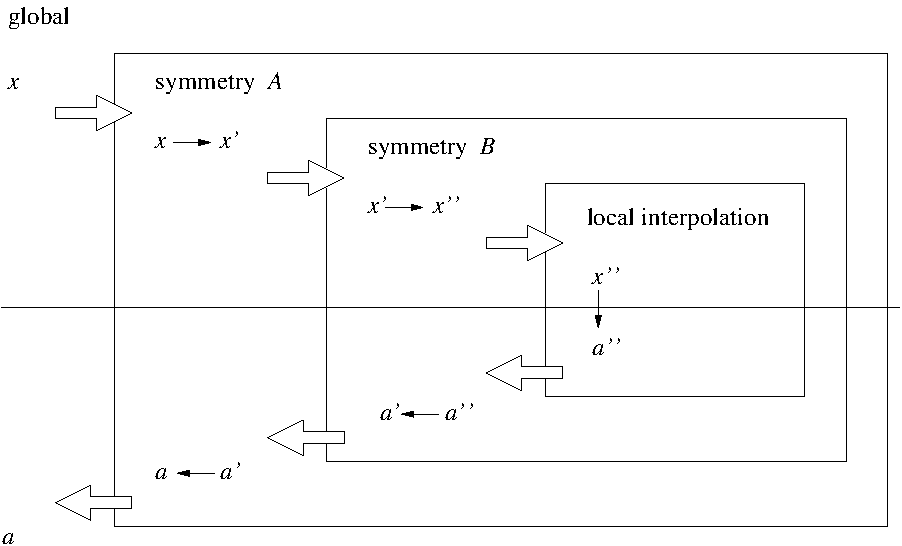
\includegraphics[scale=.833,clip=true]{fig/recursion}
\end{center}
\caption[Symmetry interpolation] {
	  The recursive calls involved in symmetry interpolation.
	  Values of grid functions $a$ at global Cartesian coordinates $x$ are 
	  calculated by nested calls to the symmetry interpolators, which first
	  apply the symmetry transformation to the coordinates.  When all
	  the symmetries have been applied, the local interpolator is called,
	  producing the interpolation of grid function values in the local basis.
	  As the symmetry interpolators return, they apply the inverse basis
	  transformation to the interpolated grid function values.
}
\label{SymBase.recursion}
\end{figure}

This mechanism has thus four players:
\begin{itemize}
	\item The driver forwards any \texttt{CCTK\_InterpGridArrays} call
	  to SymBase \texttt{SymmetryInterpolate} so that the list of
	  interpolation points can be mapped into the domain. (See section
	  \ref{SymBase.driver_interaction}.)
	\item Thorn SymBase controls which symmetry conditions perform this
	  mapping on which faces.
	\item Each symmetry boundary condition has to register a ``symmetry
	  interpolation'' routine that first maps the points into the domain,
	  then calls SymBase \texttt{SymmetryInterpolateFaces} recursively.
	  Before returning, it performs the inverse coordinate transformation
	  on the interpolated quantities.
	\item The user calls \texttt{CCTK\_InterpGridArrays}.  For them
	  the rest of the mechanism is transparent.
\end{itemize}



\subsection{Interaction With Symmetry Conditions}

The symmetry conditions have to register their ``symmetry
interpolation'' routines by calling SymBase's aliased function
\texttt{SymmetryRegisterGridInterpolator}.  The ``symmetry
interpolation'' routine must use C linkage and must have the prototype

\begin{verbatim}
CCTK_INT symmetry_interpolate
    (CCTK_POINTER_TO_CONST IN cctkGH,
     CCTK_INT IN N_dims,
     CCTK_INT IN local_interp_handle,
     CCTK_INT IN param_table_handle,
     CCTK_INT IN coord_system_handle,
     CCTK_INT IN N_interp_points,
     CCTK_INT IN interp_coords_type,
     CCTK_POINTER_TO_CONST ARRAY IN interp_coords,
     CCTK_INT IN N_input_arrays,
     CCTK_INT ARRAY IN input_array_indices,
     CCTK_INT IN N_output_arrays,
     CCTK_INT ARRAY IN output_array_types,
     CCTK_POINTER ARRAY IN output_arrays,
     CCTK_INT IN faces)
\end{verbatim}

These arguments are the same as those for \texttt{CCTK\_InterpGridArrays},
except that here the bit field \texttt{faces} is used to flag those faces
that remain to have their symmetry boundary condition applied to the
interpolation points. 

The aliased function \texttt{SymmetryRegisterGridInterpolator} has the
prototype

\begin{verbatim}
CCTK_INT FUNCTION                                           \
    SymmetryRegisterGridInterpolator                        \
        (CCTK_POINTER IN cctkGH,                            \
         CCTK_INT IN sym_handle,                            \
         CCTK_INT CCTK_FPOINTER IN symmetry_interpolate     \
             (CCTK_POINTER_TO_CONST IN cctkGH,              \
              CCTK_INT IN N_dims,                           \
              CCTK_INT IN local_interp_handle,              \
              CCTK_INT IN param_table_handle,               \
              CCTK_INT IN coord_system_handle,              \
              CCTK_INT IN N_interp_points,                  \
              CCTK_INT IN interp_coords_type,               \
              CCTK_POINTER_TO_CONST ARRAY IN interp_coords, \
              CCTK_INT IN N_input_arrays,                   \
              CCTK_INT ARRAY IN input_array_indices,        \
              CCTK_INT IN N_output_arrays,                  \
              CCTK_INT ARRAY IN output_array_types,         \
              CCTK_POINTER ARRAY IN output_arrays,          \
              CCTK_INT IN faces))
\end{verbatim}

which takes a function pointer to the aforementioned ``symmetry
interpolation'' routine, while \texttt{sym\_handle} specifies which
symmetry condition this routine is for.  This handle must have been
obtained from \texttt{SymmetryRegister}.

\begin{quote}
  The routine \texttt{SymmetryRegisterGridInterpolator} must be called
  \emph{after} the symmetry faces have been selected by the call to
  \texttt{SymmetryRegisterGrid}.
\end{quote}

For convenience, the macro \texttt{CCTK\_ALL\_FACES} is provided.
It may be used to initialize the \texttt{faces} bit field in cases
where the interpolation is to occur on all grid faces.

After it has removed from the \texttt{faces} variable the faces whose
symmetry condition it has applied, the symmetry interpolator routine
must call the SymBase function \texttt{SymmetryInterpolateFaces}, which
has the prototype

\begin{verbatim}
CCTK_INT FUNCTION                                           \
    SymmetryInterpolateFaces                                \
        (CCTK_POINTER_TO_CONST IN cctkGH,                   \
         CCTK_INT IN N_dims,                                \
         CCTK_INT IN local_interp_handle,                   \
         CCTK_INT IN param_table_handle,                    \
         CCTK_INT IN coord_system_handle,                   \
         CCTK_INT IN N_interp_points,                       \
         CCTK_INT IN interp_coords_type,                    \
         CCTK_POINTER_TO_CONST ARRAY IN interp_coords,      \
         CCTK_INT IN N_input_arrays,                        \
         CCTK_INT ARRAY IN input_array_indices,             \
         CCTK_INT IN N_output_arrays,                       \
         CCTK_INT ARRAY IN output_array_types,              \
         CCTK_POINTER ARRAY IN output_arrays,               \
         CCTK_INT IN faces)
\end{verbatim}



\subsection{Driver Interaction}
\label{SymBase.driver_interaction}

The driver has to call SymBase's aliased function
\texttt{SymmetryInterpolate}, and has to provide an aliased function
\texttt{DriverInterpolate}.  Both functions have prototypes similar to 
\texttt{CCTK\_InterpGridArrays}:

\begin{verbatim}
CCTK_INT FUNCTION
    SymmetryInterpolate
        (CCTK_POINTER_TO_CONST IN cctkGH,
         CCTK_INT IN N_dims,
         CCTK_INT IN local_interp_handle,
         CCTK_INT IN param_table_handle,
         CCTK_INT IN coord_system_handle,
         CCTK_INT IN N_interp_points,
         CCTK_INT IN interp_coords_type,
         CCTK_POINTER_TO_CONST ARRAY IN interp_coords,
         CCTK_INT IN N_input_arrays,
         CCTK_INT ARRAY IN input_array_indices,
         CCTK_INT IN N_output_arrays,
         CCTK_INT ARRAY IN output_array_types,
         CCTK_POINTER ARRAY IN output_arrays)
\end{verbatim}

\begin{verbatim}
CCTK_INT FUNCTION
    DriverInterpolate
        (CCTK_POINTER_TO_CONST IN cctkGH,
         CCTK_INT IN N_dims,
         CCTK_INT IN local_interp_handle,
         CCTK_INT IN param_table_handle,
         CCTK_INT IN coord_system_handle,
         CCTK_INT IN N_interp_points,
         CCTK_INT IN interp_coords_type,
         CCTK_POINTER_TO_CONST ARRAY IN interp_coords,
         CCTK_INT IN N_input_arrays,
         CCTK_INT ARRAY IN input_array_indices,
         CCTK_INT IN N_output_arrays,
         CCTK_INT ARRAY IN output_array_types,
         CCTK_POINTER ARRAY IN output_arrays)
\end{verbatim}


\section{Tensor Types}

Cactus supports declaring the \emph{tensor type} of grid function
groups.  These tensor types define how the grid functions, which are
supposed to be tensor components, transform under various
transformations, such as reflections and rotations.

The tensor types are not declared directly; instead, a \emph{tensor
type alias} is declared.  The following tensor type aliases are
currently known and supported:
\begin{description}
\item[\texttt{scalar}:] a scalar $\rho$
\item[\texttt{u}:] a vector $\beta^i$
\item[\texttt{d}:] a covector $s_i$
\item[\texttt{dd\_sym}:] a symmetric rank two tensor $\gamma_{ij}$
\end{description}
(More tensor type aliases are likely to be defined in the future.)

In addition to the tensor type, one can also declare the \emph{tensor
  parity}, \emph{tensor weight}, and a \emph{tensor metric}.  The
tensor parity (an integer) specifies the behaviour under reflections.
Scalars and polar vectors have a parity $+1$, pseudo scalars and axial
vectors have a parity $-1$.  The tensor weight (a real number)
specifies the behaviour under transformations that change the volume
element.  The tensor metric (a string) specifies what metric has to be
used to raise or lower indices for that quantity.

Last but not least, a \emph{tensor special} can be defined for
quantities that do not transform as tensor.  The currently supported
tensor specials are
\begin{description}
\item[\texttt{Gamma}:]
   for the transformation behaviour of the $\Gamma^i$ variables of the
   BSSN formalism; it is $\Gamma^i := - \gamma^{jk} \Gamma^i_{jk}$
   with $\Gamma^i_{jk} := \frac{1}{2} \gamma^{il} \left( \partial_k
   \gamma_{lj} + \partial_j \gamma_{lk} - \partial_l \gamma_{jk}
   \right)$
\item[\texttt{log}:]
   for the transformation behaviour of the variable $\phi$ of the BSSN
   formalism; it is $\phi := \log \psi$ with $\psi^{12} := \det
   \gamma_{ij}$.
\end{description}

By default, the basis with respect to which the tensor components are
given is supposed to be the (local) coordinate system given by the
grid, i.e., the coordinate directions are the ``natural'' directions
of the grid.  It is possible to specify a different basis by declaring
a \emph{tensor basis}, which is the name of a grid function group
containing the coordinate system.

\subsection{Example Tensor Type Declarations}

From CactusWave/WaveToy:
\begin{verbatim}
CCTK_REAL scalarevolve TYPE=gf TAGS='tensortypealias="scalar"'
\end{verbatim}

From CactusEinstein/ADMBase:
\begin{verbatim}
CCTK_REAL metric TYPE=gf TAGS='tensortypealias="dd_sym" tensormetric="ADMBase::metric"'
CCTK_REAL curv TYPE=gf TAGS='tensortypealias="dd_sym" tensormetric="ADMBase::metric"'
CCTK_REAL lapse TYPE=gf TAGS='tensortypealias="scalar" tensormetric="ADMBase::metric"'
CCTK_REAL shift TYPE=gf TAGS='tensortypealias="U" tensormetric="ADMBase::metric"'
\end{verbatim}

From AEIThorns/BSSN\_MoL:
\begin{verbatim}
CCTK_REAL ADM_BSSN_B TYPE=gf \
    TAGS='tensortypealias="u" tensormetric="ADMBase::metric"'
CCTK_REAL ADM_BSSN_dtlapse TYPE=gf \
    TAGS='tensortypealias="scalar" tensormetric="ADMBase::metric"'
CCTK_REAL ADM_BSSN_phi TYPE=gf \
    TAGS='tensortypealias="scalar" tensormetric="BSSN_MoL::ADM_BSSN_metric" \
          tensorweight=0.16666666666666667 tensorspecial="log"'
CCTK_REAL ADM_BSSN_metric TYPE=gf \
    TAGS='tensortypealias="dd_sym" tensormetric="BSSN_MoL::ADM_BSSN_metric" \
          tensorweight=-0.66666666666666667'
CCTK_REAL ADM_BSSN_K TYPE=gf \
    TAGS='tensortypealias="scalar" tensormetric="BSSN_MoL::ADM_BSSN_metric"'
CCTK_REAL ADM_BSSN_curv TYPE=gf \
    TAGS='tensortypealias="dd_sym" tensormetric="BSSN_MoL::ADM_BSSN_metric" \
          tensorweight=-0.66666666666666667'
CCTK_REAL ADM_BSSN_gamma TYPE=gf \
    TAGS='tensortypealias="u" tensormetric="BSSN_MoL::ADM_BSSN_metric" \
          tensorweight=0.66666666666666667 tensorspecial="Gamma"'
\end{verbatim}

% Do not delete next line
% END CACTUS THORNGUIDE

\end{document}
